% \documentclass{IEEEtran} 
\documentclass{IEEEconf} 
\usepackage{url}
% \usepackage{hyperref}
\usepackage{amssymb,amsmath}
\usepackage{pdfpages}
\usepackage{graphicx}

\title{No solution? Clustering to Evaluate Multiple Imputation } 
\author{Anthony S. Chapman, Dr Steven Turner, Dr. Wei Pang} 
\begin{document} 
	\maketitle{} 

% Glad I could help. You already have a quarter of a paper. 
% Some initial comments:
% Personally, I would do the discussion before the conclusion, or incorporate the two together as Discussion and Conclusion. Remember - don't use colloquial language.
% Also, you want to head a section as The Problem to make it abundantly clear what it is. You need to lead them by the nose. You must always explain what you are going to tell them, tell them what you are going to tell them, then tell them what you have told them to get the message across -subtly, of course. Expand Acronyms the first time you use them. Also, explain everything if you want the paper to appeal to a wider audience. If you write for an audience who understand all the language, great for them, but if you want to refer to it later for a different audience, better to make it super clear and lead them by the hand.

% Anyway - you are off and running. Good luck - you'll have three papers in no time at all.

% There is nothing to easily compare different imputation techniques, post researches haven't got computing background... (need a way to formally say that statement, maybe number of disciplines VS computing?? ) 

	\abstract{Blah}

	\section{Introduction} % (fold)
	\label{sec:introduction}
		Data collection has been increasing 
		Missing data is inevitable (human and computing reasons, i.e. people not putting it in or computer corrupting it, )
		Non-computing people either imputate willy-neely or ignore missing data - need to use as much data as you can. (Ask Graham about theory about using as much data as possible for better analysis)
		Many imputation algorithms out there with many parameters, which is best? 
		Need 
	% section introduction (end)

	\section{Background} % (fold)
	\label{sec:background}
		Talk about something \cite{epi1}
		\cite{bigData}
	% section background (end)

	\section{The Problems} % (fold)
	\label{sec:the_problem}
		\subsection{Incompleteness} % (fold)
		\label{sub:incompleteness}
			With so many new data being collected daily \cite{bigData}, it was inevitable that some of the data would have missing values \cite{missing1}, whether they be through human error or computational inefficiency. Although there are ways to combat missing data such as mean-value imputation or multiple imputation \cite{missing1,missing2,missing3}, many researchers whom are not very computational or statistically confident would rather disregard any records with missing values \cite{epi1,ep2,ep3,ep4,ep5}. As an example, in \cite{epi1}, the authors decided to use 2,758 records for analysis out of the possible 44,261 mainly due to missing data, this is a mere 6.2\% out of the records available. There must be a way for even non-computing or non-statistical researchers to benefit from the tools available. 
		% subsection incompleteness (end)
		\subsection{Will it work on my data?} % (fold)
		\label{sub:will_it_work_on_my_data_}
			This next problem arises when a researchers does decide to use the data with missing values but does not have sufficient knowledge to apply the available methods, like Muliple Imputation by Chained Equations (MICE \cite{mice}) using the computational language R \cite{r} or the Impute Missing Values function in the statistical software SPSS \cite{spss}. The problem is, how do you know if the imputed values are representative to the truth, how do you know whether record 2,754 column 5 is male or not after you apply the imputation method.

			Even if the imputation method has been proven to work on someone else's dataset such as \cite{compare}, this no indication it will work for yours, unless you have the exact dataset as them, which is unrealistic. This is due to the many reasons and ways that missing data is creates, for example there might be a relationship between one missing value and another one. 

			In order to test whether an imputation method works on your dataset, you need something to compare the results to, a benchmark, like this one would be able to analyse what effect of the methods. Unfortunately, it is very difficult to find a complete dataset which contains the same characteristics of your own dataset, there will always be differences. 
		% subsection will_it_work_on_my_data_ (end)
		\subsection{Which imputation is best for me} % (fold)
		\label{sub:which_imputation_is_best_for_me}
			The following problem applies to researchers, even those computationally competent, who wish to find out whether one imputation method is better than another. There is nothing to easily compare results from different imputation methods or same imputation methods with slightly different parameters. The main problem arises when one tries to compare the outcomes from one method to another, here an adequate analogy would be that compare imputation method A to method B would be like comparing chocolate with a bicycle; the outcomes might not be comparable. 

			There should a way to compare different methods without having to create your own computer software in the process. Although 
		% subsection which_imputation_is_best_for_me (end)
	% section the_problem (end)

	\section{Possible Solutions} % (fold)
	\label{sec:a_solution}
		\subsection{Incompleteness} % (fold)
		\label{sub:incompleteness}
			Imputation will create values where there were non before, one has to be careful when imputing data as there are many techniques (default value, mean value and multiple imputation just to name a few) as using them without care will lead to erroneous data \cite{careful}. By creating a user-friendly program with clear guidelines on how to use it and some explanation on how it works, we believe that researchers whom would normally ignore data with missing values will be more likely to use more of their data through imputation. 
		% subsection incompleteness (end)
		\subsection{Testing your own data} % (fold)
		\label{sub:testing_your_own_data}
			In order to test how well an imputation technique, such as MICE, you need to be able to compare the effects of the imputation method to a benchmark, we propose creating a benchmark from the users own dataset. By analysing the missing data characteristics, extracting the subset of complete data from the dataset and then replicating the same dataset onto the subset, we are able to create artificial mini datasets which behave as the original one except now we have a benchmark to compare the effects of imputation. 

		% Use your own level or missingness as a benchmark and create mini-me's as bench-mark. You are the closest thing to yourself. 
		% Group theory stuff, multidimensional-mixed data distance measurements, Gower, medoids, widths and dissimilarities.

		% Just because it worked on someone else, doesn't mean it works for you, cite papers who test specific datasets. 

		% subsection testing_your_own_data (end)
		\subsection{Comparing Imputations} % (fold)
		\label{sub:comparing_imputations}
			In order for a researcher to be able to compare different imputation techniques on their own datasets, the outcomes of the techniques need to ``talk the same language''. By having a program that takes a dataset and imputation pair and then outputs the efficiency of the imputation, one is able to compare these outputs with ease and without having to understand the individual imputation technique outputs. 

			% Will now be able to compare different imputations on your own dataset with ``normalised '' results for comparison. 
		% subsection comparing_imputations (end)
	% section a_solution (end)
	\section{The Framework} % (fold)
	\label{sec:the_framework}

		\begin{figure}[!ht]
			\caption{Framework flowchart}
			\centering
			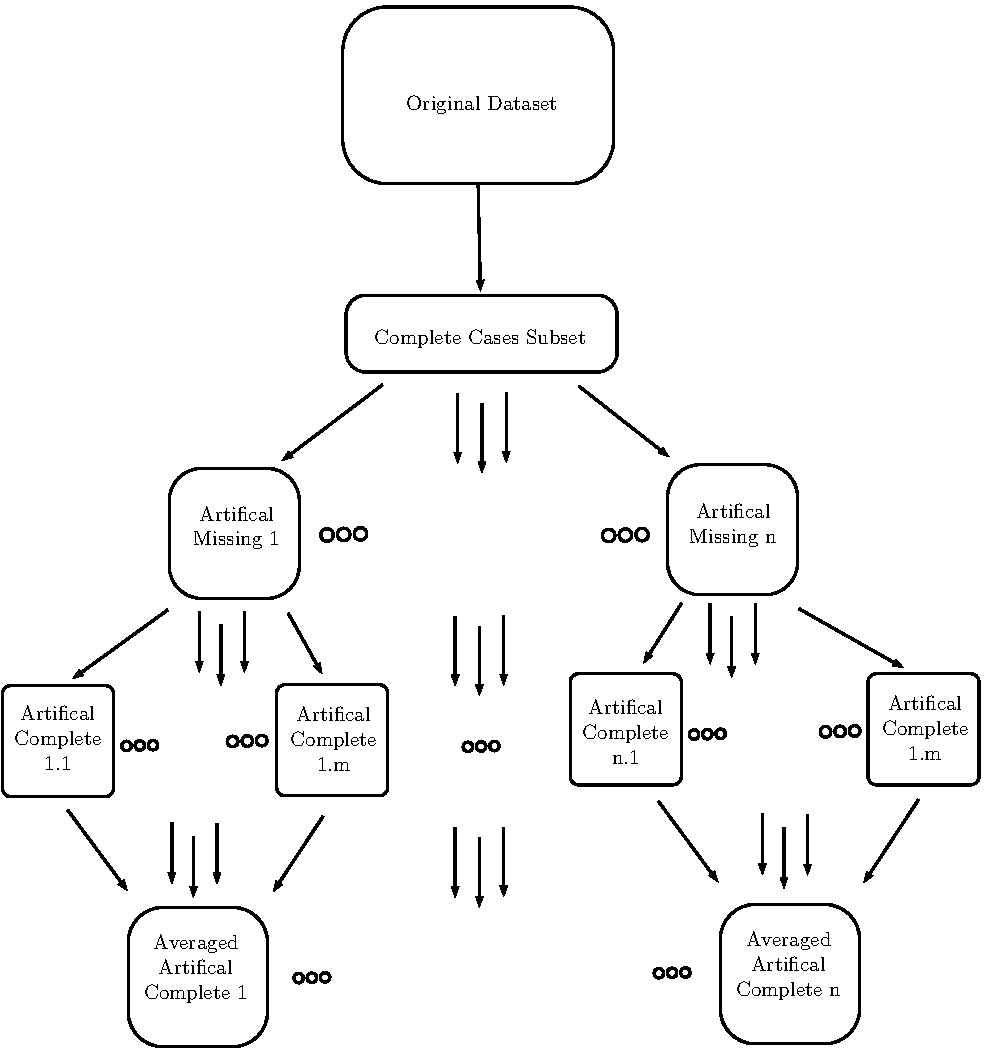
\includegraphics[width=0.5\textwidth]{diagram.pdf}
		\end{figure}
		The process is as follows: Using a dataset with missing values, call this ``OD'', for original dataset, and an imputation technique, call this ``Imp'', you first analyse the missingness characteristics of ``OD'' to in order to apply them later. Then, create a new dataset by deleting any record from ``OD'', call this "CC", for complete cases. Using the missingness characteristics, we create more da

		The proposed framework is as follows: In order to assess the effects of any imputation technique, the program will need a dataset with missing values, called ``D'', and an imputation method, called ``I''. Then the function ``I(x)'' is a function that takes a data with missing values and outputs an imputed dataset. 

		Specify dataset (O) and imputation method (I)
		Analyse dataset to obtain the missing characteristics
		Create subset of dataset with only complete cases (C)
		Apply missing characteristics to create n individual datasets out of C, called ($ArtM_{1}, ArtM_{2}...ArtM_{n}$)
		Impute all $Art_{n}$ to created artificially complete datasets $ArtC_{n}$
		Apply clustering algorithm to C and all $ArtC_{n}$ to create $ClustC$ and $ClustArt_{n}$
		Average clustering outcomes from all $ClusArt_{n}$ and compare to $ClustC$
		Analyse how far the average of all $ClusArt_{n}$ have gone from $ClustC$
		Normalise the distance to give a percentage of goodness for the user.
	% section the_framework (end)

	\section{Conclusion} % (fold)
	\label{sec:conclusion}
	It's better to use all the data you can but can't blindly imputation. This framework indicates whether your data 
	% section conclusion (end)

	\section{Discussion} % (fold)
	\label{sec:discussion}
	Working on implementing this, ClEMI, any researcher regardless the computing ability will be able to use it. 
	% section discussion (end)

	\bibliographystyle{plain}
	\bibliography{papers}

\end{document}



The first step will be to analyse the original dataset to find the missing value characteristics. We then great a dataset out of the original one by deleting all the records with missing values in it. The next step will be to create n amount of artificial datasets 